% CSE 715 — Computer Graphics
% Chapter 2: Image Representation — Complete Model Answers (2020–2024)
% University of Chittagong, 7th Semester B.Sc. Engineering
% Source: Schaum's Outline of Computer Graphics (Xiang & Plastock), Chapter 2, pp.7-24
%
% Compile with: pdflatex Chapter2_Solutions.tex (run twice for TOC)

\documentclass[12pt, a4paper]{article}

\usepackage[left=2.5cm, right=2.5cm, top=2.8cm, bottom=2.8cm, headheight=15pt]{geometry}
\usepackage{amsmath, amssymb}
\usepackage{tikz}
\usetikzlibrary{arrows.meta, positioning, shapes.geometric, calc, backgrounds, fit}
\usepackage{booktabs}
\usepackage{array}
\usepackage{xcolor}
\usepackage{enumitem}
\usepackage{fancyhdr}
\usepackage{titlesec}
\usepackage{mdframed}
\usepackage{multicol}
\usepackage{tabularx}
\usepackage{multirow}
\usepackage{hyperref}

%----- Colours -----
\definecolor{sectionblue}{RGB}{10,60,110}
\definecolor{boxbg}{RGB}{242,247,255}
\definecolor{answerbg}{RGB}{240,255,240}
\definecolor{notesbg}{RGB}{255,250,230}
\definecolor{keyblue}{RGB}{0,80,160}
\definecolor{accent}{RGB}{180,40,40}

%----- Box environments -----
\mdfdefinestyle{solutionframe}{linecolor=sectionblue, backgroundcolor=boxbg, roundcorner=4pt, linewidth=1.4pt, innertopmargin=7pt, innerbottommargin=7pt, innerleftmargin=9pt, innerrightmargin=9pt}
\mdfdefinestyle{answerframe}{linecolor=green!55!black, backgroundcolor=answerbg, roundcorner=4pt, linewidth=1.4pt, innertopmargin=7pt, innerbottommargin=7pt, innerleftmargin=9pt, innerrightmargin=9pt}
\mdfdefinestyle{notesframe}{linecolor=orange!70!black, backgroundcolor=notesbg, roundcorner=4pt, linewidth=1pt, innertopmargin=5pt, innerbottommargin=5pt, innerleftmargin=8pt, innerrightmargin=8pt}
\newenvironment{solutionbox}{\begin{mdframed}[style=solutionframe]}{\end{mdframed}}
\newenvironment{answerbox}{\begin{mdframed}[style=answerframe]}{\end{mdframed}}
\newenvironment{notesbox}{\begin{mdframed}[style=notesframe]}{\end{mdframed}}

%----- Page style -----
\pagestyle{fancy}
\fancyhf{}
\lhead{\small\color{sectionblue} CSE 715 — Chapter 2: Image Representation}
\rhead{\small\color{sectionblue} Model Solutions (2020--2024)}
\cfoot{\small\thepage}
\renewcommand{\headrulewidth}{0.5pt}

%----- Section formatting -----
\titleformat{\section}{\Large\bfseries\color{sectionblue}}{}{0em}{}[\vspace{-2pt}\color{sectionblue}\rule{\linewidth}{0.8pt}]
\titleformat{\subsection}{\large\bfseries\color{sectionblue!85!black}}{}{0em}{}
\titleformat{\subsubsection}{\normalsize\bfseries\color{black}}{}{0em}{}

%----- Custom list -----
\newlist{keypoints}{itemize}{1}
\setlist[keypoints]{label=$\triangleright$, leftmargin=1.5cm, itemsep=2pt, topsep=3pt}
\newlist{examlist}{enumerate}{1}
\setlist[examlist]{label=\textbf{(\roman*)}, leftmargin=1.8cm, itemsep=3pt, topsep=4pt}

%=====================================================================
\begin{document}
%=====================================================================

\begin{center}
  {\LARGE\bfseries\color{sectionblue} CSE 715: Computer Graphics}\\[0.6em]
  {\Large\bfseries Chapter 2 --- Image Representation}\\[0.3em]
  {\large Complete Model Answers (2020--2024)}\\[0.2em]
  {\normalsize University of Chittagong \quad|\quad 7\textsuperscript{th} Semester B.Sc.\ (Engg.) Examination}\\[0.3em]
  {\small Source: Schaum's Outline of Computer Graphics (Xiang \& Plastock), Chapter 2, pp.7--24}
\end{center}

\vspace{0.3em}
\noindent\rule{\linewidth}{1pt}
\vspace{0.5em}

\tableofcontents
\newpage

%=====================================================================
\section{Theoretical Framework --- Reusable Across All Years}
%=====================================================================
This section covers the \textbf{core theory} that appears in every year's Q1 (and often spills into Q2/Q3). Master these once — every year's Chapter 2 question is a re-mix of the same handful of ideas.

%----------------------------------------------------------------------
\subsection{Computer Graphics vs. Image Processing}
%----------------------------------------------------------------------
\begin{center}
\renewcommand{\arraystretch}{1.4}
\begin{tabular}{p{4cm}|p{6cm}|p{6cm}}
\toprule
& \textbf{Computer Graphics} & \textbf{Image Processing} \\
\midrule
\textbf{Starting point} & An abstract object definition (in object space) & An existing image (in image space) \\
\textbf{Operation} & Synthesis --- object $\to$ image & Pixel-based transformation --- image $\to$ image \\
\textbf{Goal} & Create a picture from a model & Enhance/analyse/modify a picture that already exists \\
\textbf{Example} & Rendering a 3D scene from vertex data & Sharpening, denoising, or recoloring a photograph \\
\bottomrule
\end{tabular}
\end{center}
\begin{answerbox}
\textbf{One-liner (memorise):} Computer Graphics goes \emph{object $\to$ image}; Image Processing goes \emph{image $\to$ image}. Computer--Human Interaction (HCI) is the third allied field --- it studies effective communication between user and machine (input devices, GUIs), overlapping with CG mainly at graphical user interfaces.
\end{answerbox}

\subsubsection*{How a digital image is formed from an object definition (the graphics pipeline)}
\begin{center}
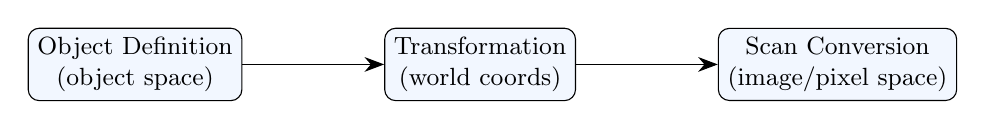
\begin{tikzpicture}[node distance=1.6cm, every node/.style={font=\small}]
  \node[draw, rounded corners, fill=boxbg, align=center] (rep) {Object Definition\\(object space)};
  \node[draw, rounded corners, fill=boxbg, align=center, right=1.8cm of rep] (trans) {Transformation\\(world coords)};
  \node[draw, rounded corners, fill=boxbg, align=center, right=1.8cm of trans] (scan) {Scan Conversion\\(image/pixel space)};
  \draw[-{Stealth[length=2.5mm]}] (rep) -- (trans);
  \draw[-{Stealth[length=2.5mm]}] (trans) -- (scan);
\end{tikzpicture}
\end{center}
A shape (e.g.\ a triangle's vertex coordinates) is defined abstractly in \textbf{object space} (continuous), placed/scaled/rotated into the \textbf{world coordinate system} via \textbf{transformation} (matrices), then \textbf{scan-converted} (rasterized) into discrete pixels in \textbf{image space}.

%----------------------------------------------------------------------
\subsection{The RGB and CMY Color Models}
%----------------------------------------------------------------------
\begin{keypoints}
  \item \textbf{RGB (additive):} Start from \textbf{black} $(0,0,0)$, \emph{add} Red/Green/Blue light to reach the desired color. White $=(1,1,1)$. Matches how a \textbf{display monitor} works (emits light).
  \item \textbf{CMY (subtractive):} Start from \textbf{white} $(0,0,0)$ in CMY-space, \emph{subtract} (absorb) primaries using Cyan/Magenta/Yellow pigment to reach the desired color. Black $=(1,1,1)$ in CMY. Matches how a \textbf{printer} works (pigments absorb light reflected off paper).
  \item \textbf{Conversion formulas:}
  $$\begin{pmatrix}R\\G\\B\end{pmatrix} = \begin{pmatrix}1\\1\\1\end{pmatrix} - \begin{pmatrix}C\\M\\Y\end{pmatrix} \qquad\qquad \begin{pmatrix}C\\M\\Y\end{pmatrix} = \begin{pmatrix}1\\1\\1\end{pmatrix} - \begin{pmatrix}R\\G\\B\end{pmatrix}$$
  \item \textbf{Why printers add a 4th, black (K) pigment (CMYK):} producing a deep, pure black by mixing C+M+Y is technically difficult (tends toward muddy brown) and \textbf{more expensive} (uses 3 costly color pigments instead of 1 cheap black one) than using a dedicated black ink.
\end{keypoints}

\subsubsection*{Perceptual color terms vs. physical light properties}
\begin{center}
\renewcommand{\arraystretch}{1.3}
\begin{tabular}{l|l}
\toprule
\textbf{Perceptual term} & \textbf{Physical property of light} \\
\midrule
\textbf{Hue} & Dominant wavelength \\
\textbf{Saturation (Purity)} & Excitation purity --- how "undiluted" by white light the color is \\
\textbf{Brightness (Lightness/Value)} & Luminance / intensity \\
\bottomrule
\end{tabular}
\end{center}

%----------------------------------------------------------------------
\subsection{Direct Coding}
%----------------------------------------------------------------------
Direct coding allocates a fixed number of bits per pixel to code its color \textbf{directly} — no indirection. If $n_r, n_g, n_b$ bits are used for R, G, B respectively:
\begin{answerbox}
$$\text{number of colors per pixel} = 2^{n_r}\times 2^{n_g}\times 2^{n_b}$$
If all three primaries use the same $n$ bits: $\text{colors} = (2^n)^3 = 2^{3n}$.
\end{answerbox}
Special cases: \textbf{bilevel} (black/white) images need only 1 bit/pixel; \textbf{gray-scale} images typically use 8 bits/pixel (256 levels), coded once since R=G=B. The industry-standard \textbf{24-bit "true color"} format uses 1 byte (8 bits, 256 levels) per primary $\Rightarrow 256^3 = 16.7$ million colors.

%----------------------------------------------------------------------
\subsection{Lookup Table (LUT)}
%----------------------------------------------------------------------
Instead of coding color directly, each pixel stores an \textbf{address/index} into a table of colors (the \emph{color map}). An $n$-bit pixel value indexes a table of $2^n$ entries; each entry typically holds a full 24-bit RGB color.
\begin{answerbox}
$$\text{LUT entries} = 2^{(\text{bits per pixel})} \qquad\qquad \text{LUT storage (bits)} = 2^{(\text{bits per pixel})}\times(\text{bits per entry})$$
\end{answerbox}
\textbf{Trade-off:} LUT gives a smaller storage footprint (e.g.\ 8-bit pixel + 24-bit table = "8-bit format", 256 simultaneous colors chosen from 16.7M) at the cost of only $2^n$ \emph{simultaneous} colors in one image, vs.\ direct coding's full color range being available pixel-by-pixel.

%----------------------------------------------------------------------
\subsection{Aspect Ratio, Resizing, and Sub-Image Cropping}
%----------------------------------------------------------------------
\begin{answerbox}
\textbf{Aspect ratio} $= \dfrac{\text{width}}{\text{height}}$ (unit length or pixels). \\
\textbf{Resize without distortion} requires the \emph{new} aspect ratio to equal the \emph{original} aspect ratio: $\dfrac{w_1}{h_1} = \dfrac{w_2}{h_2}$. If they differ, the image is stretched/squeezed — \textbf{geometric distortion} occurs. \\
\textbf{Center-crop a $w\times h$ sub-image from a $W\times H$ image:} lower-left corner of the crop in the big image $= \left(\dfrac{W-w}{2}, \dfrac{H-h}{2}\right)$; upper-right corner $=$ lower-left $+\,(w,h)$.
\end{answerbox}

%----------------------------------------------------------------------
\subsection{Halftoning, Halftone Approximation, and Dithering}
%----------------------------------------------------------------------
\begin{keypoints}
  \item \textbf{Halftoning:} a printing-industry technique using \textbf{variably-sized} pigment dots (arranged at a $45^\circ$ screen angle) that, viewed from a distance, blend with the white background to simulate continuous-tone shading on a \textbf{bilevel} device. Dot size $\propto$ intensity level (bigger dot $\to$ darker perceived tone).
  \item \textbf{Halftone approximation:} instead of varying dot \emph{size}, use an $n\times n$ grid of \textbf{fixed-size} bilevel (or multi-level) pixels turned on in a specific growth pattern to approximate the look of variable dot sizes.
  \begin{answerbox}
  With an $n\times n$ pixel grid where each pixel can take $m$ intensity levels: $$\text{overall intensity levels} = n\times n\times(m-1) + 1$$ (the "+1" accounts for the all-off / zero-intensity level.)
  \end{answerbox}
  \item \textbf{Dither matrix:} an $n\times n$ matrix $D_n$ that encodes the \emph{order} in which grid pixels are turned on. Pixel $(x,y)$ is turned on if the image's intensity level at that position exceeds $D_n(i,j)$ where $i = x \bmod n$, $j = y \bmod n$ (the matrix "tiles" across the whole image like floor tiles — this is called \textbf{dithering}, and it approximates halftones \emph{without} sacrificing spatial resolution).
  \item \textbf{Recurrence relation to build a bigger dither matrix from a smaller one} (Bayer matrix construction):
  $$D_{2n} = \begin{pmatrix} 4D_n & 4D_n+2 \\ 4D_n+3 & 4D_n+1 \end{pmatrix}$$
\end{keypoints}

%=====================================================================
\section{Examination 2024 --- Q2, Q3 (Section A)}
%=====================================================================

\begin{solutionbox}
\textbf{Question breakdown:}
\begin{enumerate}[noitemsep]
  \item[Q2(a)] Explain the concept of a color model and why RGB/CMY are both used. (3)
  \item[Q2(b)] Crop 128$\times$128 from the center of a 512$\times$512 image --- upper-left corner coords. (2)
  \item[Q2(c)] 10-bit grayscale pixel values in a LUT --- entries required. (1)
  \item[Q2(d)] What is halftoning; how does it create continuous-tone appearance. (3)
  \item[Q3(a)] Given a halftone-pattern image, describe how dot size/spacing changes create intensity perception. (2)
  \item[Q3(b)] Given $D_2=\begin{pmatrix}0&2\\3&1\end{pmatrix}$ and the recurrence, construct $D_4$. (3)
\end{enumerate}
\end{solutionbox}

\subsection*{Q2(a) --- Color Model Concept [3 marks]}
See \S1.2 above. \textbf{Key point:} RGB matches \emph{emissive} devices (monitors, additive mixing of light); CMY matches \emph{reflective} devices (printers, subtractive absorption of light from ambient/incident light). Both are needed because graphics content must round-trip between screen (RGB) and print (CMY).

\subsection*{Q2(b) --- Crop Coordinates [2 marks]}
\begin{answerbox}
Upper-left corner in the big image $= \left(\dfrac{512-128}{2}, \dfrac{512-128}{2}\right) = (192, 192)$.
\end{answerbox}

\subsection*{Q2(c) --- LUT Entries [1 mark]}
\begin{answerbox}
$10$-bit pixel values $\Rightarrow 2^{10} = \mathbf{1024}$ entries required.
\end{answerbox}

\subsection*{Q2(d) --- What is Halftoning [3 marks]}
See \S1.6. Halftoning uses variable dot size at a fixed grid pitch; larger dots reflect less white paper $\to$ perceived as darker; smaller dots $\to$ perceived as lighter. Viewed from normal reading distance, the eye cannot resolve individual dots and integrates them into a smooth gray-level gradient.

\subsection*{Q3(a) --- Halftone Pattern Description [2 marks]}
As intensity increases across the gradient, dot \textbf{size grows} (occupying more of each cell) while center-to-center \textbf{spacing (pitch) stays fixed} — larger dots merge visually, reducing the fraction of visible white background, which the eye reads as a smooth transition from light to dark.

\subsection*{Q3(b) --- Construct $D_4$ from $D_2$ [3 marks]}
\begin{solutionbox}
$$D_2 = \begin{pmatrix}0&2\\3&1\end{pmatrix}, \qquad D_4 = \begin{pmatrix}4D_2 & 4D_2+2\\ 4D_2+3 & 4D_2+1\end{pmatrix}$$
$$4D_2=\begin{pmatrix}0&8\\12&4\end{pmatrix},\quad 4D_2{+}2=\begin{pmatrix}2&10\\14&6\end{pmatrix},\quad 4D_2{+}3=\begin{pmatrix}3&11\\15&7\end{pmatrix},\quad 4D_2{+}1=\begin{pmatrix}1&9\\13&5\end{pmatrix}$$
\end{solutionbox}
\begin{answerbox}
$$D_4 = \begin{pmatrix} 0 & 8 & 2 & 10\\ 12 & 4 & 14 & 6\\ 3 & 11 & 1 & 9\\ 15 & 7 & 13 & 5 \end{pmatrix}$$
(This is the well-known $4\times4$ \textbf{Bayer ordered-dither matrix} — recognise it on sight.)
\end{answerbox}

%=====================================================================
\section{Examination 2023 --- Q1 (Section A, parts a/b/g of 9)}
%=====================================================================

\begin{solutionbox}
\textbf{Question breakdown (Q1 is 9$\times$1 = 9 marks total, a--i):}
\begin{enumerate}[noitemsep]
  \item[(a)] How can you differentiate computer graphics from image processing? (1)
  \item[(b)] Crop a 786$\times$660 sub-image from the center of a 1200$\times$1200 image --- lower-left \& upper-right pixel coords. (1)
  \item[(g)] Name the three perceptual terms for describing color \& the corresponding physical property of light. (1)
\end{enumerate}
\emph{(Parts c--f, h, i of Q1 2023 belong to other topics --- projection/hidden-surface/color-transform clusters; not repeated here.)}
\end{solutionbox}

\subsection*{Q1(a) --- CG vs. Image Processing [1 mark]}
See \S1.1 --- CG: object $\to$ image; Image Processing: image $\to$ image.

\subsection*{Q1(b) --- Crop Coordinates [1 mark]}
\begin{answerbox}
Lower-left $= \left(\dfrac{1200-786}{2}, \dfrac{1200-660}{2}\right) = (207, 270)$. \\
Upper-right $=$ lower-left $+ (786, 660) = (993, 930)$.
\end{answerbox}

\subsection*{Q1(g) --- Perceptual Color Terms [1 mark]}
\begin{answerbox}
\textbf{Hue} $\leftrightarrow$ dominant wavelength; \textbf{Saturation} $\leftrightarrow$ purity of the color (how little it's diluted by white); \textbf{Brightness} $\leftrightarrow$ luminance/intensity of the light.
\end{answerbox}

%=====================================================================
\section{Examination 2022 --- Q1 (Section A, parts a--f)}
%=====================================================================

\begin{solutionbox}
\textbf{Question breakdown:}
\begin{enumerate}[noitemsep]
  \item[(a)] How do CG, Image Processing, and Human-Computer Interaction differ? (implicit within Q1)
  \item[(b)] Resize a 1680$\times$1050 image to 1024 wide, same aspect ratio --- new height? (2)
  \item[(c)] 2-byte pixel values in a LUT representation --- bits occupied? (1)
  \item[(d)] Direct coding of CMY: 3 bits cyan, 3 bits magenta, 4 bits yellow --- possible colors per pixel? (1)
  \item[(e)] Can a 5$\times$3.5in image be shown at 3.5$\times$4in without geometric distortion? (2)
  \item[(f)] Why do color printers use a subtractive color model? (1)
\end{enumerate}
\end{solutionbox}

\subsection*{Q1(b) --- Resize Preserving Aspect Ratio [2 marks]}
\begin{answerbox}
$\text{height} = 1024 \times \dfrac{1050}{1680} = \mathbf{640}$ pixels.
\end{answerbox}

\subsection*{Q1(c) --- LUT Bits Occupied [1 mark]}
\begin{answerbox}
2-byte (16-bit) pixel $\Rightarrow 2^{16} = 65{,}536$ entries. If each entry is a standard 24-bit RGB value: $65{,}536 \times 24 = \mathbf{1{,}572{,}864}$ bits ($=196{,}608$ bytes).
\end{answerbox}

\subsection*{Q1(d) --- Direct Coding CMY, Mixed Bit Widths [1 mark]}
\begin{answerbox}
$2^3 \times 2^3 \times 2^4 = 8 \times 8 \times 16 = \mathbf{1024}$ possible colors.
\end{answerbox}

\subsection*{Q1(e) --- Distortion Check [2 marks]}
\begin{answerbox}
Original AR $= 5/3.5 = 1.4286$. Target AR $= 3.5/4 = 0.875$. Not equal $\Rightarrow$ \textbf{No}, distortion occurs (the image will appear stretched/squeezed).
\end{answerbox}

\subsection*{Q1(f) --- Why Subtractive Model for Printers [1 mark]}
Printers deposit pigment that \textbf{absorbs} certain wavelengths of ambient/reflected light rather than emitting light directly — this passive, reflective process is inherently subtractive (start from white paper, subtract color), unlike a monitor which actively emits RGB light (additive).

%=====================================================================
\section{Examination 2021 --- Q1 (Section A, parts a--e)}
%=====================================================================

\begin{solutionbox}
\textbf{Question breakdown:}
\begin{enumerate}[noitemsep]
  \item[(a)] How does image processing differ from computer graphics? Briefly explain. (1)
  \item[(b)] 2-byte pixel values in a 24-bit LUT representation --- bits occupied? (1.25)
  \item[(c)] Direct coding RGB, 12 bits per primary color --- possible colors per pixel? (1)
  \item[(d)] Resize a 1024$\times$675 image onto two devices: 800$\times$527 and 1800$\times$1100 --- what phenomena occur, with computation. (3)
  \item[(e)] Crop a 700$\times$700 sub-image from the center of a 900$\times$800 image --- upper-right corner coords. (1.5)
\end{enumerate}
\emph{(Part f, the Koch curve, belongs to the Scan Conversion/Fractals topic --- covered separately.)}
\end{solutionbox}

\subsection*{Q1(b) --- LUT Bits Occupied [1.25 marks]}
\begin{answerbox}
$2^{16} \times 24 = \mathbf{1{,}572{,}864}$ bits.
\end{answerbox}

\subsection*{Q1(c) --- Direct Coding, 12 bits/primary [1 mark]}
\begin{answerbox}
$2^{12} \times 2^{12} \times 2^{12} = 2^{36} = \mathbf{68{,}719{,}476{,}736}$ possible colors.
\end{answerbox}

\subsection*{Q1(d) --- Resize onto Two Devices [3 marks]}
\begin{solutionbox}
Original AR $= 1024/675 = 1.51704$. \\
Device (a) $800\times527$: AR $= 800/527 = 1.51803$ --- within $\sim 0.07\%$ of original: \textbf{negligible distortion}, image displays essentially correctly. \\
Device (b) $1800\times1100$: AR $= 1800/1100 = 1.63636$ --- roughly $7.9\%$ off from original: \textbf{noticeable geometric distortion} (image appears stretched wider relative to its height).
\end{solutionbox}
\begin{answerbox}
\textbf{(a)} Near-zero distortion (AR essentially matches). \textbf{(b)} Visible distortion --- the picture looks stretched because the device's aspect ratio doesn't match the image's.
\end{answerbox}

\subsection*{Q1(e) --- Crop Coordinates [1.5 marks]}
\begin{answerbox}
Lower-left $= \left(\dfrac{900-700}{2}, \dfrac{800-700}{2}\right) = (100, 50)$. \\
Upper-right $=$ lower-left $+ (700,700) = (800, 750)$.
\end{answerbox}

%=====================================================================
\section{Examination 2020 --- Q1, Q2 (Group-A, parts a--d and a--c)}
%=====================================================================

\begin{solutionbox}
\textbf{Question breakdown:}
\begin{enumerate}[noitemsep]
  \item[Q1(a)] Which discipline describes producing and synthesizing digital images? Justify. (3)
  \item[Q1(b)] Can a 5$\times$3.5in image be presented at 3.5$\times$4in without geometric distortion? (2)
  \item[Q1(c)] How can a digital image be formed from an object definition? (1.25)
  \item[Q1(d)] Why is a standard aspect ratio necessary? Height $=2$in, AR$=1.5$ --- find width. (1+1.5)
  \item[Q2(a)] What do you mean by subtractive color model? Give an example. Why do printers use a separate black cartridge? (1+1)
  \item[Q2(b)] Direct coding RGB, 10 bits/primary --- possible colors per pixel? (1.5)
  \item[Q2(c)] Crop 700$\times$700 from the center of a 900$\times$800 image --- upper-right corner coords. (2.75)
\end{enumerate}
\emph{(Q2(d), flood-fill, belongs to the Scan Conversion topic --- covered separately.)}
\end{solutionbox}

\subsection*{Q1(a) --- Discipline Identification [3 marks]}
\begin{answerbox}
\textbf{Computer Graphics.} Justification: it is the field concerned with generating and synthesizing digital images from geometric/object definitions, as opposed to capturing images from the real world (photography) or processing existing images (image processing).
\end{answerbox}

\subsection*{Q1(b) --- Distortion Check [2 marks]}
\begin{answerbox}
AR original $=5/3.5=1.4286$; AR target $=3.5/4=0.875$. Not equal $\Rightarrow$ distortion occurs.
\end{answerbox}

\subsection*{Q1(c) --- Digital Image Formation [1.25 marks]}
See the pipeline diagram in \S1.1: Object Definition $\to$ Transformation $\to$ Scan Conversion.

\subsection*{Q1(d) --- Aspect Ratio Necessity + Width Calc [1+1.5 marks]}
A standard aspect ratio must be maintained so images display without geometric distortion across devices of different physical dimensions/resolutions.
\begin{answerbox}
Width $= \text{AR}\times\text{height} = 1.5\times 2 = \mathbf{3}$ inches.
\end{answerbox}

\subsection*{Q2(a) --- Subtractive Color Model [1+1 marks]}
\begin{answerbox}
\textbf{Subtractive model:} start from white, \emph{subtract} (absorb) primary components using pigment to reach a color; e.g.\ \textbf{CMY} (cyan, magenta, yellow) used by printers. \textbf{Why a separate black cartridge:} mixing full C+M+Y to make black is costly (three expensive pigments) and technically hard to get a true, deep black (tends muddy) — a dedicated black (K) ink is cheaper and gives cleaner text/blacks.
\end{answerbox}

\subsection*{Q2(b) --- Direct Coding, 10 bits/primary [1.5 marks]}
\begin{answerbox}
$2^{10}\times 2^{10}\times 2^{10} = \mathbf{1{,}073{,}741{,}824}$ possible colors.
\end{answerbox}

\subsection*{Q2(c) --- Crop Coordinates [2.75 marks]}
\begin{answerbox}
Lower-left $=(100,50)$, upper-right $=(800,750)$ --- identical setup to 2021 Q1(e) above.
\end{answerbox}

%=====================================================================
\section{Quick Summary --- Exam Patterns for Chapter 2}
%=====================================================================

\begin{center}
\renewcommand{\arraystretch}{1.3}
\begin{tabular}{p{5.5cm}|p{2.5cm}|p{6cm}}
\toprule
\textbf{Pattern} & \textbf{Years} & \textbf{Formula / Method to memorise} \\
\midrule
Center-crop sub-image coords & every year & lower-left $=\left(\frac{W-w}{2},\frac{H-h}{2}\right)$, upper-right $=$ lower-left $+(w,h)$ \\
Direct coding bit $\to$ color count & every year & colors $=2^{n_r}\times2^{n_g}\times2^{n_b}$ \\
LUT entries/bits & every year & entries $=2^{\text{bits/pixel}}$; storage $=$ entries $\times$ bits/entry \\
Aspect-ratio distortion check & every year & compare $w_1/h_1$ vs.\ $w_2/h_2$ --- equal $=$ no distortion \\
CG vs. Image Processing & every year & object$\to$image (CG) vs.\ image$\to$image (IP) \\
Subtractive/CMY reasoning & 2020, 2022, 2023 & printers absorb light (subtractive); K added for cost + true black \\
Halftoning \& dither matrix & 2024 only (new) & recurrence $D_{2n}=\begin{pmatrix}4D_n&4D_n+2\\4D_n+3&4D_n+1\end{pmatrix}$ \\
\bottomrule
\end{tabular}
\end{center}

\begin{notesbox}
\textbf{Exam-day strategy for Q1/Q2 (Chapter 2 cluster):} this is almost always a fast, low-risk 8--13 marks if you drill the five formulas above cold — every sub-part is a 1--3 mark plug-and-compute, not a derivation. Spend no more than 15--20 minutes of exam time here; bank the marks early and move to the heavier Ch4/Ch5/Ch7/Ch10 questions.
\end{notesbox}

\end{document}
